\documentclass[a4paper]{article}

\usepackage{amsmath,amsfonts,amsthm,amssymb,mathtools} % Math packages
\usepackage[utf8]{inputenc} % Required for non-English characters
\usepackage[english]{babel} % Spell-checking
\usepackage{fancyhdr} % Required for custom headers
\usepackage{lastpage} % Required to determine the last page for the footer
\usepackage{extramarks} % Required for header and footer marks
\usepackage[margin=1.2in]{geometry} % Sets page margin
\usepackage{esdiff} % Defines commands for differentials
\mathtoolsset{showonlyrefs} % Only referenced equations are numbered
\usepackage{xfrac} % Allows for slanted fractions using \sfrac{*}{*}
\usepackage{graphicx} % For pictures
\usepackage{float}
\usepackage{siunitx}
\usepackage[arrowdel]{physics}
\usepackage{mdframed} % boxing answers
\AtBeginDocument{\RenewCommandCopy\qty\SI}
\usepackage{bm}

% The following sets up the header and footer
\fancyhf{}
\pagestyle{fancy}
\lhead{\hmwkCourse} %left header
\rhead{\hmwkTitle \, \textendash \, \hmwkName \, \textendash \, \hmwkClass} % right header
\rfoot{Page\ \thepage\ of\ \pageref{LastPage}} % right footer
\renewcommand\headrulewidth{0.4pt} % Size of the header rule
\renewcommand\footrulewidth{0.4pt} % Size of the footer rule

% The following sets the information shown in header and footer
\newcommand{\hmwkTitle}{Homework 3} % Assignment title
\newcommand{\hmwkCourse}{Optics} % Course/class
\newcommand{\hmwkName}{John Meneghini} % Your name
\newcommand{\hmwkClass}{2/26/2024}

% The following sets new paragraphs to start with a line skip instead of an indentation. Just my preference.
\setlength{\parindent}{0pt} %No indentation of new paragraphs
\setlength{\parskip}{10pt}

\begin{document}

\section*{Question 1}
A beam of light in air strikes the surface of a smooth piece of plastic having an index of refraction 1.55 at an angle of incidence of \ang{20}. The incident light has an electric field with component parallel to the plane of incidence of \qty{10}{V \per m} and component perpendicular to the plane of incidence of \qty{20}{V \per m}. Determine the corresponding reflected electric field amplitudes. \\\\

As derived in class, for the component parallel to the plane of incidence:

\[
    r_\parallel = \frac{E_{r, \parallel}}{E_{i, \parallel}} = \frac{n_t \cos \theta_i - n_i \cos \theta_t}{n_i \cos \theta_t + n_t \cos \theta_i}
\]

and 

\[
    r_\perp = \frac{E_{r, \perp}}{E_{i, \perp}} = \frac{n_i \cos \theta_i - n_t \cos \theta_t}{n_i \cos \theta_i + n_t \cos \theta_t},
\]

where $n_i = 1.00$, $n_t = 1.55$, $\theta_i = \ang{20}$, and 

\[
    \theta_t = \sin^{-1}\left(\frac{n_i \sin \theta_i}{n_t}\right) = \ang{12.75}.
\]

Thus,

\[
    r_\parallel = 0.198,
\]

and

\[
    r_\perp = -0.233.
\]

Considering the amplitudes,

\[
    E_{r, \parallel} = r_\parallel E_{i, \parallel} = 0.198 (\qty{10}{V \per m}) = \qty{1.98}{V \per m},
\]

and

\[
    E_{r, \perp} = r_\perp E_{i, \perp} = 0.233 (\qty{20}{V \per m}) = \qty{4.67}{V \per m}
\]
\newpage
\section*{Question 2}

\begin{figure}[H]
    \centering
    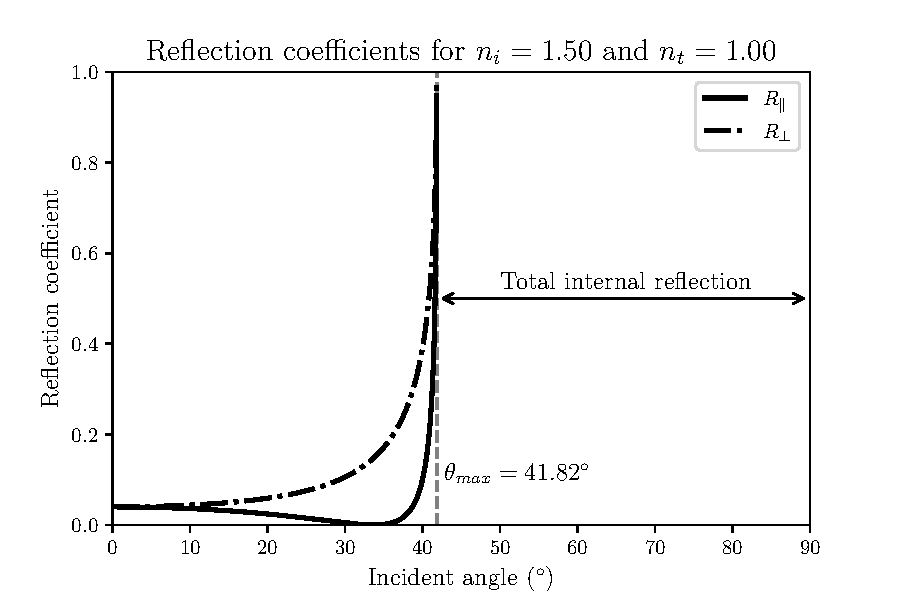
\includegraphics[width = \textwidth]{reflection_coefficients.pdf}
    \caption{$R_\parallel$ and $R_\perp$ for $n_i = 1.5$ and $n_t = 1.0$.}
\end{figure}

\section*{Question 3}
Show that
\[
    T_\parallel = \frac{\sin 2 \theta_i \sin 2 \theta_t}{\sin^2 (\theta_i + \theta_t) \cos^2 (\theta_i - \theta_t)}
\]
and
\[
    T_\perp = \frac{\sin 2 \theta_i \sin 2 \theta_t}{\sin^2(\theta_i + \theta_t)}
\] \\

\begin{align}
    T_\parallel &= \frac{n_t \cos \theta_t}{n_i \cos \theta_i} t_\parallel^2 = \frac{n_t \cos \theta_t}{n_i \cos \theta_i} \frac{4 n_i^2 \cos^2 \theta_i}{n_t^2 \cos^2 \theta_i + n_i^2\cos^2 \theta_t + 2 n_i n_t \cos \theta_i \cos \theta_t}\\
    &=\frac{4 n_i n_t \cos \theta_i \cos \theta_t}{n_t^2 \cos^2 \theta_i + n_i^2\cos^2 \theta_t + 2 n_i n_t \cos \theta_i \cos \theta_t}\\
    &=\frac{4\left(\frac{n_i^2 \sin \theta_i}{\sin \theta_t}\right)\cos \theta_i \cos \theta_t}{\frac{n_i^2 \sin^2 \theta_i}{\sin^2 \theta_t} \cos^2 \theta_i + n_i^2 \cos^2 \theta_t + 2\left(\frac{n_i^2 \sin \theta_i}{\sin \theta_t}\right)\cos \theta_i \cos \theta_t} \left( \frac{\sin^2 \theta_t}{\sin^2 \theta_t} \right)\\
    &=\frac{\sin 2 \theta_i \sin 2 \theta_t}{\frac{1}{4}\sin^2 2 \theta_i + \frac{1}{4}\sin^2 2 \theta_t + \frac{1}{2}\sin 2 \theta_i \sin 2 \theta_t} = \frac{\sin 2 \theta_i \sin 2 \theta_t}{\frac{1}{4}\left(\sin 2 \theta_i  + \sin 2 \theta_t\right)^2}\\
    &=  \frac{\sin 2 \theta_i \sin 2 \theta_t}{\sin^2 (\theta_i + \theta_t) \cos^2 (\theta_i - \theta_t)}
\end{align}

and

\begin{align}
    T_\perp &= \frac{n_t \cos \theta_t}{n_i \cos \theta_i} t_\perp^2 = \frac{n_t \cos \theta_t}{n_i \cos \theta_i} \frac{4 n_i^2 \cos^2 \theta_i}{n_i^2 \cos^2 \theta_i + n_t^2\cos^2 \theta_t + 2 n_i n_t \cos \theta_i \cos \theta_t}\\
    &=\frac{4 n_i n_t \cos \theta_i \cos \theta_t}{n_i^2 \cos^2 \theta_i + n_t^2\cos^2 \theta_t + 2 n_i n_t \cos \theta_i \cos \theta_t}\\
    &=\frac{4\left(\frac{n_i^2 \sin \theta_i}{\sin \theta_t}\right)\cos \theta_i \cos \theta_t}{n_i^2\cos^2 \theta_i + \frac{n_i^2 \sin^2 \theta_i}{\sin^2 \theta_t} \cos^2 \theta_t + 2\left(\frac{n_i^2 \sin \theta_i}{\sin \theta_t}\right)\cos \theta_i \cos \theta_t} \left( \frac{\sin^2 \theta_t}{\sin^2 \theta_t} \right)\\
    &=\frac{\sin 2 \theta_i \sin 2 \theta_t}{\cos^2 \theta_i \sin^2 \theta_t + \cos^2 \theta_t \sin^2 \theta_i + \frac{1}{2}\sin 2 \theta_i \sin 2 \theta_t}\\
    &=\frac{\sin 2 \theta_i \sin 2 \theta_t}{\sin^2 (\theta_i + \theta_t)}
\end{align}
\section*{Question 4}
Show that
\[
    R_\parallel  + T_\parallel = 1
\]
and
\[
    R_\perp  + T_\perp = 1
\]\\\\

For $R_\parallel  + T_\parallel = 1$,

\begin{align}
    R_\parallel  + T_\parallel &= r_\parallel^2 + \frac{n_t \cos \theta_t}{n_i \cos \theta_i}t_\parallel^2 = \left(\frac{n_i \cos \theta_t - n_t \cos \theta_i}{n_i \cos \theta_t + n_t \cos \theta_i}\right)^2 + \frac{n_t \cos \theta_t}{n_i \cos \theta_i}\frac{4 n_i^2 \cos^2 \theta_i}{(n_i \cos \theta_t + n_t \cos \theta_i)^2}\\
    &= \frac{n_i^2 \cos^2 \theta_t + n_t^2 \cos^2 \theta_i - 2 n_i n_t \cos \theta_i \cos \theta_t + 4 n_i n_t \cos \theta_i \cos \theta_t}{(n_i \cos \theta_t + n_t \cos \theta_i)^2}\\
    &= \frac{n_i^2 \cos^2 \theta_t + n_t^2 \cos^2 \theta_i + 2 n_i n_t \cos \theta_i \cos \theta_t}{(n_i \cos \theta_t + n_t \cos \theta_i)^2}\\
    &= \frac{(n_i \cos \theta_t + n_t \cos \theta_i)^2}{(n_i \cos \theta_t + n_t \cos \theta_i)^2} = 1
\end{align}

Now for $R_\perp  + T_\perp = 1$,

\begin{align}
    R_\perp  + T_\perp &= r_\perp^2 + \frac{n_t \cos \theta_t}{n_i \cos \theta_i}t_\perp^2 = \left(\frac{n_i \cos \theta_i - n_t \cos \theta_t}{n_i \cos \theta_i + n_t \cos \theta_t}\right)^2 + \frac{n_t \cos \theta_t}{n_i \cos \theta_i} \frac{4 n_i^2 \cos^2 \theta_i}{\left(n_i \cos \theta_i + n_t \cos \theta_t\right)^2}\\
    &= \frac{n_i^2 \cos^2 \theta_i + n_t^2 \cos^2 \theta_t - 2 n_i n_t \cos \theta_i \cos \theta_t + 4 n_i n_t \cos \theta_i \cos \theta_t}{\left(n_i \cos \theta_i + n_t \cos \theta_t\right)^2}\\
    &= \frac{n_i^2 \cos^2 \theta_i + n_t^2 \cos^2 \theta_t + 2 n_i n_t \cos \theta_i \cos \theta_t}{\left(n_i \cos \theta_i + n_t \cos \theta_t\right)^2}\\
    &=\frac{\left(n_i \cos \theta_i + n_t \cos \theta_t\right)^2}{\left(n_i \cos \theta_i + n_t \cos \theta_t\right)^2} = 1
\end{align}

\section*{Question 5}
Show that 
\[
    \grad({\ln \abs{\va*{r}}}) = \frac{\va*{r}}{r^2}
\]\\

In spherical coordinates,

\[
    \grad(f(r, \theta, \varphi)) = \pdv{f}{r} \vu*{r} + \frac{1}{r} \pdv{f}{\theta} \vu*{\theta} + \frac{1}{r \sin \theta}\pdv{f}{\varphi} \vu*{\varphi}.
\]

Thus,

\[
    \grad(\ln \abs{\va*{r}}) = \grad(\ln r) =  \vu*{r}\pdv{r} \ln r = \frac{\vu*{r}}{r} = \frac{\va*{r}}{r^2}.
\]





\end{document}